%% Creator: Inkscape inkscape 0.48.0, www.inkscape.org
%% PDF/EPS/PS + LaTeX output extension by Johan Engelen, 2010
%% Accompanies image file 'param_vs_dir_res.eps' (pdf, eps, ps)
%%
%% To include the image in your LaTeX document, write
%%   \input{<filename>.pdf_tex}
%%  instead of
%%   \includegraphics{<filename>.pdf}
%% To scale the image, write
%%   \def\svgwidth{<desired width>}
%%   \input{<filename>.pdf_tex}
%%  instead of
%%   \includegraphics[width=<desired width>]{<filename>.pdf}
%%
%% Images with a different path to the parent latex file can
%% be accessed with the `import' package (which may need to be
%% installed) using
%%   \usepackage{import}
%% in the preamble, and then including the image with
%%   \import{<path to file>}{<filename>.pdf_tex}
%% Alternatively, one can specify
%%   \graphicspath{{<path to file>/}}
%% 
%% For more information, please see info/svg-inkscape on CTAN:
%%   http://tug.ctan.org/tex-archive/info/svg-inkscape

\begingroup
  \makeatletter
  \providecommand\color[2][]{%
    \errmessage{(Inkscape) Color is used for the text in Inkscape, but the package 'color.sty' is not loaded}
    \renewcommand\color[2][]{}%
  }
  \providecommand\transparent[1]{%
    \errmessage{(Inkscape) Transparency is used (non-zero) for the text in Inkscape, but the package 'transparent.sty' is not loaded}
    \renewcommand\transparent[1]{}%
  }
  \providecommand\rotatebox[2]{#2}
  \ifx\svgwidth\undefined
    \setlength{\unitlength}{224.4984375pt}
  \else
    \setlength{\unitlength}{\svgwidth}
  \fi
  \global\let\svgwidth\undefined
  \makeatother
  \begin{picture}(1,1.89401722)%
    \put(0,0){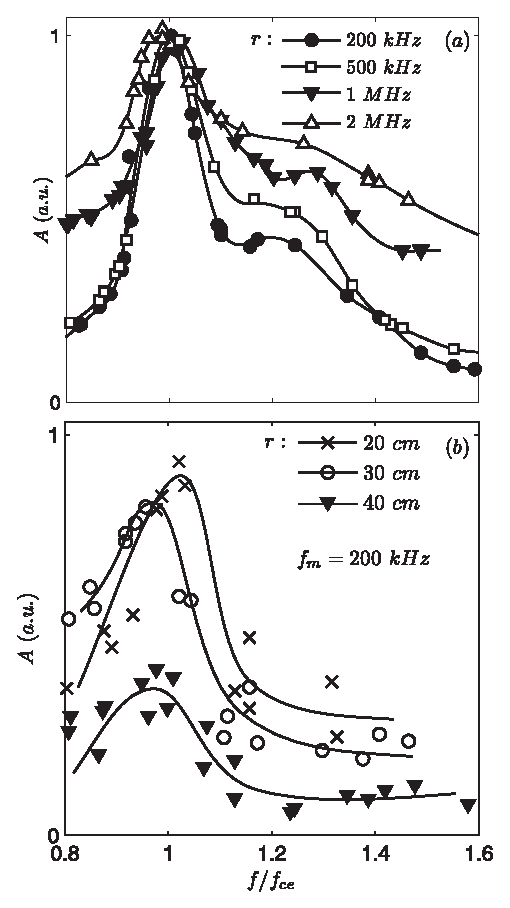
\includegraphics[width=\unitlength]{pics/param_vs_dir_res.eps}}%
    \put(0.06,1.73){\color[rgb]{0,0,0}\makebox(0,0)[lb]{\smash{$1$}}}%
    \put(0.06,0.97){\color[rgb]{0,0,0}\makebox(0,0)[lb]{\smash{$0$}}}%
    \put(0.06,0.05){\color[rgb]{0,0,0}\makebox(0,0)[lb]{\smash{$0$}}}%
    \put(0.06,0.89){\color[rgb]{0,0,0}\makebox(0,0)[lb]{\smash{$1$}}}%
    \put(0.0687818,0.01){\color[rgb]{0,0,0}\makebox(0,0)[lb]{\smash{$0.8$}}}%
    \put(0.308,0.01){\color[rgb]{0,0,0}\makebox(0,0)[lb]{\smash{$1$}}}%
    \put(0.504,0.01){\color[rgb]{0,0,0}\makebox(0,0)[lb]{\smash{$1.2$}}}%
    \put(0.724,0.01){\color[rgb]{0,0,0}\makebox(0,0)[lb]{\smash{$1.4$}}}%
    \put(0.95,0.01){\color[rgb]{0,0,0}\makebox(0,0)[lb]{\smash{$1.6$}}}%
    \put(0.46547512,-0.06){\color[rgb]{0,0,0}\makebox(0,0)[lb]{\smash{$f/f_{ce}$}}}%
    \put(0.58,0.65){\color[rgb]{0,0,0}\makebox(0,0)[lb]{\smash{$f_m=200$\,кГц}}}%

    \put(0.75,0.748){\color[rgb]{0,0,0}\makebox(0,0)[lb]{\smash{$40$\,см}}}%
    \put(0.75,0.812){\color[rgb]{0,0,0}\makebox(0,0)[lb]{\smash{$30$\,см}}}%
    \put(0.75,0.874){\color[rgb]{0,0,0}\makebox(0,0)[lb]{\smash{$20$\,см}}}%
    \put(0.51,0.874){\color[rgb]{0,0,0}\makebox(0,0)[lb]{\smash{$r:$}}}%
    \put(0.5,1.723){\color[rgb]{0,0,0}\makebox(0,0)[lb]{\smash{$r:$}}}%   
    \put(0.03,0.45){\color[rgb]{0,0,0}\rotatebox{90}{\makebox(0,0)[lb]{\smash{$A$\,(у.е.)}}}}%
    \put(0.03,1.3){\color[rgb]{0,0,0}\rotatebox{90}{\makebox(0,0)[lb]{\smash{$A$\,(у.е.)}}}}%
    \put(0.88,0.88){\color[rgb]{0,0,0}\makebox(0,0)[lb]{\smash{$(б)$}}}%
    \put(0.88,1.72){\color[rgb]{0,0,0}\makebox(0,0)[lb]{\smash{$(а)$}}}%
    \put(0.713,1.548){\color[rgb]{0,0,0}\makebox(0,0)[lb]{\smash{$2$\,МГц}}}%
    \put(0.713,1.6152){\color[rgb]{0,0,0}\makebox(0,0)[lb]{\smash{$1$\,МГц}}}%
    \put(0.713,1.668){\color[rgb]{0,0,0}\makebox(0,0)[lb]{\smash{$500$\,кГц}}}%
    \put(0.713,1.72){\color[rgb]{0,0,0}\makebox(0,0)[lb]{\smash{$200$\,кГц}}}%
  \end{picture}%
\endgroup
